\documentclass[paper=a4, fontsize=11pt]{scrartcl} % A4 paper and 11pt font size
\usepackage{./../usfassignment}
\settitle{Assignment 9}
\setauthor{Wanzhang Sheng}
\setcourse{CS675: Automata Theory}
\setlength\parindent{1em} % Removes all indentation from paragraphs - comment this line for an assignment with lots of text

\begin{document}

\maketitle % Print the title


% \begin{fancyquotes}
%   Question 5.4.2 from the text: Which of the following problems about
%   Turing Machines are solvable,and which are undecidable? Explain your
%   answers carefully --- if your answer is that the problem is
%   undedicable, then give a reduction that proves that it is
%   undecidable (that is, do not use Rice's Theorem). If your answer is
%   that the problem is decidable, describe how the problem could be
%   solved.
% \end{fancyquotes}

%= 1 ====================
\section{}
\begin{fancyquotes}
  (4 points) To determine, given a Turing machine $M$ and a state
  $q$, whether $M$ will ever reach a configuration with state $q$
  when started with the input $w$ from its intial state.
\end{fancyquotes}

\begin{figure}[H]
  \centering
  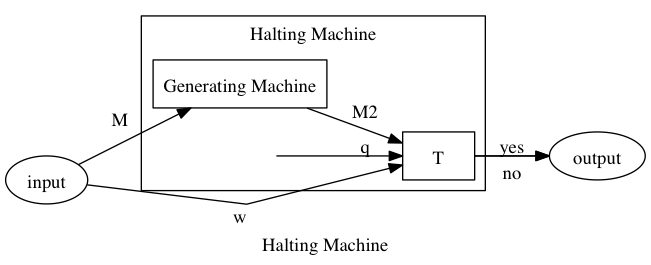
\includegraphics[width=\textwidth]{9-1.gv.png}
  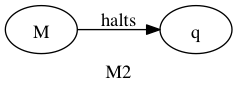
\includegraphics[width=.4\textwidth]{9-1.gv.2.png}
\end{figure}

Undecidable.

The generating machine generates $M_2$ by modified $M$, when $M$
halts transfer to a new state $q$. If machine $T$ exists, then halting
machine exists. So $T$ doesn't exist.


%= 2 ====================
\section{}
\begin{fancyquotes}
  (4 points) To determine, given a Turing machine $M$ and two
  states $p$ and $q$, whether there is any configuration with state
  $p$ which yields a configuration with state $q$.
\end{fancyquotes}

\begin{figure}[H]
  \centering
  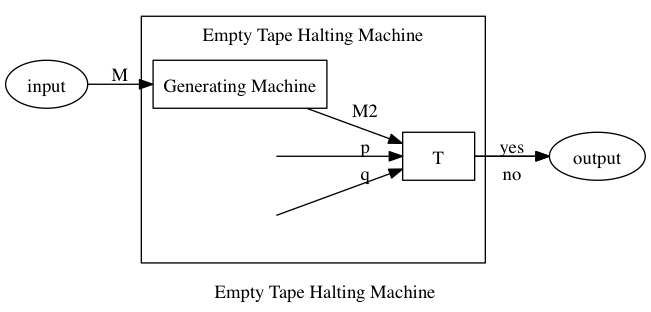
\includegraphics[width=\textwidth]{9-2.gv.png}
  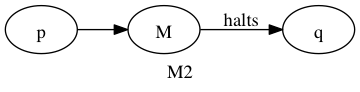
\includegraphics[width=.5\textwidth]{9-2.gv.2.png}
\end{figure}

Undecidable.

The generating machine generates $M_2$ by modified $M$. Start from
state $p$ and when $M$ halts transfer to a new state $q$. If machine
$T$ exists, then empty tape halting machine exists. So $T$ doesn't
exist.


%= 3 ====================
\section{}
\begin{fancyquotes}
  (4 points) To determine, given a Turing machine $M$ and a state
  $q$, whether there is any configuration at all that yields a
  configuration with state $q$.
\end{fancyquotes}

Decidable.

For a given TM $M$, we can search the $e(M)$ to find if it exists a
transition $(p,c)\rightarrow (q,a)$. If it exists, we can generate the
configuration of $M$ with state $p$, position $t$ and write $c$ under
$t$, so that this configuartion will lead to state $q$. If it doesn't
exist, output NO.


%= 4 ====================
\section{}
\begin{fancyquotes}
  (4 points) To determine, given a Turing machine $M$ and a symbol
  $a$, whether $M$ ever writes the symbol $a$ when started on the
  empty tape.
\end{fancyquotes}

\begin{figure}[H]
  \centering
  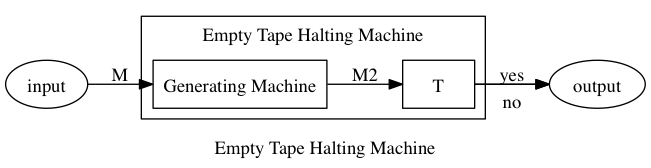
\includegraphics[width=\textwidth]{9-4.gv.png}
  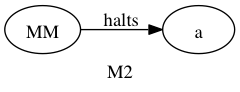
\includegraphics[width=.5\textwidth]{9-4.gv.2.png}
\end{figure}

Undecidable.

The generating machine generates $M_2$ by modified $M$. Replace all
the symbol $a$ appeared in $M$ by new symbol $x$ to get $MM$. And when
$MM$ halts transfer to a new state and write $a$. $M_2$ write $a$ when
and only when the $M$ halts on empty tape.

If machine $T$ exists, then empty tape halting machine exists. So $T$
doesn't exist.


%= 5 ====================
\section{}
\begin{fancyquotes}
  (4 points) To determine, given a Turing machine $M$, whether $M$
  ever writes $a$ nonblank symbol when started on the empty tape.
\end{fancyquotes}

Decidable.

If $M$ doesn't write any nonblank symbol with an empty tape
at the beginning, it means that the TM can only move left, move right
(write blank on an empty tape is meaningless). So if the machine
doesn't halt when a state appears twice, it will run forever and
ever. Since the machine has finite states, it can be determined in
finite steps.


%= 6 ====================
\section{}
\begin{fancyquotes}
  (4 points) To determine, given a Turing machine $M$ and a string
  $w$, whether $M$ ever moves its head to the left when started with
  input $w$.
\end{fancyquotes}

Decidable.

If a TM never move left, it means that it will never be in the same
position twice. If it is in the same position with the same symbol
under the pointer twice, it will run forever. Since the conbination of
the states and the symbols are finate, we can determine it in finite
time. Take all the blanks after the string as a single position to
determin it with the same method.


%= 7 ====================
\section{}
\begin{fancyquotes}
  (4 points) To determine, given two Turing machines, whether one
  semi-decides the complement of the language decided by the other.
\end{fancyquotes}

Undecidable.

Since the second language is decidable. We can easily create the
complement machine by reverse the output. It's also decidable.
Then the machine is trying to tell whether the first language is same
with the complement language. Since we already know $L[M_1]=L[M_2]$ is
undecidable, the original problem is also undecidable.


%= 8 ====================
\section{}
\begin{fancyquotes}
  (4 points) To determine, given two Turing machines, whether there
  is any string on whch they both halt.
\end{fancyquotes}

\begin{figure}[H]
  \centering
  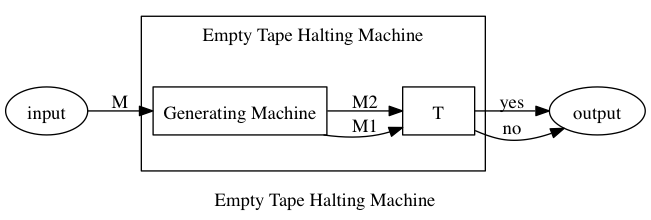
\includegraphics[width=\textwidth]{9-8.gv.png}
  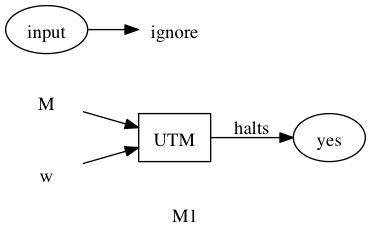
\includegraphics[width=.4\textwidth]{9-8.gv.2.png}
  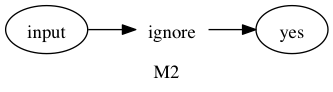
\includegraphics[width=.4\textwidth]{9-8.gv.3.png}
\end{figure}

If and only if $M$ halts on $w$, two TMs $M_1$ and $M_2$ halt on any
string. Otherwise $M_1$ run forever and halts on nothing. So we can
use $T$ to solve Empty Tape Halting Machine. Since Empty Tape Halting
Machine doesn't exist, $T$ doesn't exist. So the problem is undecidable.


%= 9 ====================
\section{}
\begin{fancyquotes}
  (4 points) To determine, given a Turing machine $M$, whether the
  language semi-decided by $M$ is finite.
\end{fancyquotes}

\begin{figure}[H]
  \centering
  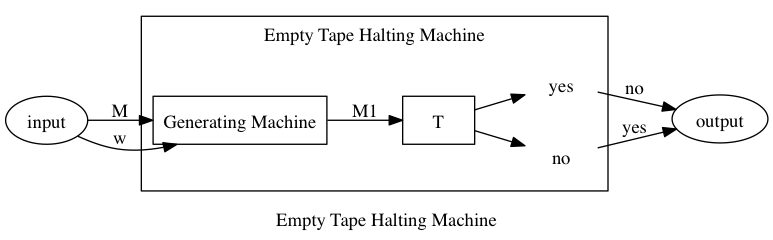
\includegraphics[width=\textwidth]{9-9.gv.png}
  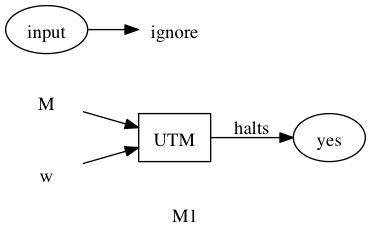
\includegraphics[width=.4\textwidth]{9-9.gv.2.png}
\end{figure}

When $M$ halts on $w$, $M_1$ output anything which means $T$ output
NO. When $M$ doesn't halt on $w$, $M_1$ output nothing which means $T$
output YES. So we can use $T$ to solve Empty Tape Halting
Machine. Since Empty Tape Halting Machine doesn't exist, $T$ doesn't
exist. So the problem is undecidable.


\end{document}
